\documentclass[twocolumn]{svjour3}[2016]

\usepackage{graphicx}
\usepackage{cite}
\usepackage{subfigure}
\usepackage{mathtools}
\usepackage{amsmath}

\begin{document}
%HEADER
\title{Exploring Unstructured Environment with Frontier Trees}
\author{Rudolf F. S. Korb \and Prof. Dr. habil. Alfred Schoettl}
\institute{
	R. F. S. Korb \at
	University of Applied Sciences - Munich\\ Dept. 04 Electrical Engineering and Information Technology, Laboratory for Autonomous Systems in Munich (LASIM),  Lothstr. 64, 80335 Munich, Germany\\Tel.: +49-89-1265-3415\\
	\email{rudolf.korb@hm.edu}
	\and
	Prof. Dr. habil. A. Schoettl \at
	University of Applied Sciences - Munich\\ Dept. 04 Electrical Engineering and Information Technology, Laboratory for Autonomous Systems in Munich (LASIM),  Lothstr. 64, 80335 Munich, Germany\\Tel.: +49-89-1265-3415\\
	\email{alfred.schoettl@hm.edu}
}

\maketitle

\begin{abstract}
\textbf{
%\textit{
	This paper presents the Frontier Tree exploration algorithm, a novel approach to autonomously explore unknown and unstructured areas. Focus of this work is the exploration of domestic environments with arbitrary obstacles, for example furbished appartements. Existing and well studied approaches like greedy algorithms perform worse, when obstacles are included and the range of distance sensors is limited. Base of this research is the Frontier Tree. This data structure offers two main features. It is a memory of past poses during exploration and is utilized to decide between future navigation goals. This approach is compared to a basic but efficient nearest neighbour exploration. The algorithm is tested in simulation with maps similar to appartement ground maps including furniture as obstacles. The paper shows, that frontier trees minimize the travelled path of the mobile robot by tracking open boundaries.

}
\keywords{Robotics \and  Exploration \and  Path Planning \and  Frontiers \and Domestic Environment}
\end{abstract}

\section{Introduction}
\label{introduction}
Mobile robots must be familiar with their surroundings to execute complex tasks, for example pick-up and delivery services. As an initial step, the workspace has to be explored autonomously. This problem can be divided into three parts; mapping, localization and exploration. Focus of this research is planning future exploration steps to uncover the environment efficiently, depending on past steps, a map of the area already explored and the agent's current position.\\
When robots participate in everyday life, their operation space consists of unstructured, dynamic environments and has to deal with interieur and crowded areas.
As a consequence, when service robots operate in private appartements or public buildings like hospitals or retirement homes, they need to adapt itselves to their surroudings.
Therefore it is crucial for a mobile robot to explore areas autonomously and not rely on an environment designed specifically for a service device.\\
Basic algorithms follow a greedy approach to select future robot positions during the exploration problem. These approaches use the robot's current state and plan one step ahead by minimizing a cost function, for example the agent's euclidian distance to a boundary of known and unknown space. For exploration of simple maps, unfurbished rooms and corridors, basic algorithms provide acceptable results, depending on for example sensor constraints. With high range distance sensors and obstacle free areas, robots cover the entire room before leaving and most likely do not create open boundaries. Therefore, rooms do not have to be visited again and the traveled distance is less compared to low range sensing robots. Furthermore, the number of possible decisions to choose the next goal from is rising with the environment's complexity. As a result, the greedy algorithm's performance will decrease. The robot has to revisit parts of the map where boundaries have been forgotten, increasing the traveled distance.\\
Consequently the two main influences for travelling distance during exploration is the complexity of an agent's environment and constraints of its range sensors. Mobile autonomous robots in unstructered environment are dealing with both, high complexity and sensor limitations. Many algorithms use maps with reduced difficulty, expecting an empty environment or assume a sensor with infinite distance measurements. It follows, that algorithms covering only one impact decrease in efficiency, when a complex environment and sensor limitations are present.\\
Greedy algorithms dealing with both influences have one major flaw, which leads to a rise of traveled distance and exploration time. Approaching a boundary already discovered several steps ahead, is an indication that the robot's current exploration path is a cycle. As a result, open boundaries between the starting and endpoint of the cycle will be reached with high travel costs later on during the exploration task. The frontier tree recognizes cycles and hence is able to avoid high costs and react early on forgotten boundaries.

% For one-column wide figures use
%\begin{figure}
%  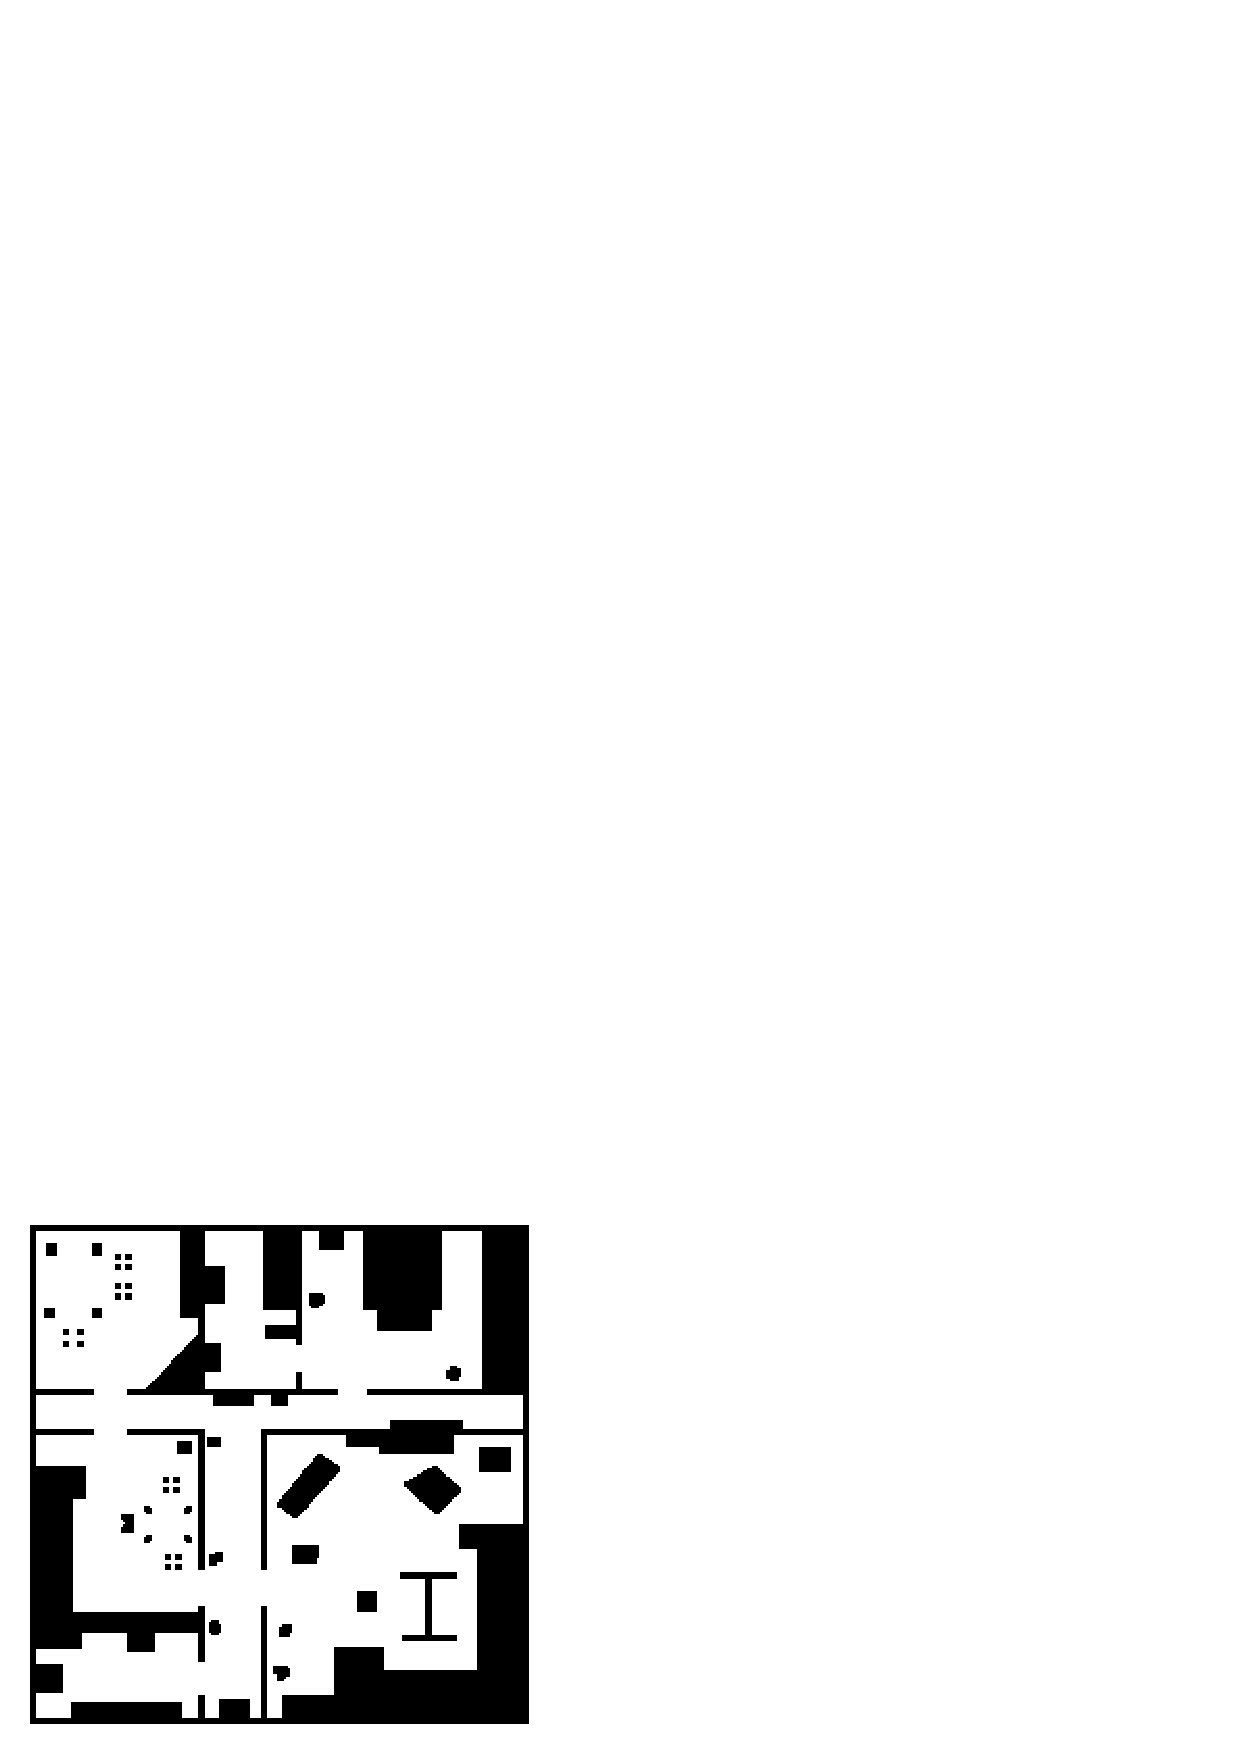
\includegraphics[width=5cm,height=5cm]{map_19.pdf}
% figure caption is below the figure
%\caption{Please write your figure caption here}
%\label{fig:1}       % Give a unique label
%\end{figure}

\section{Related Work}
\label{related_work}
Many exploration algorithms use the frontier approach introduced by Yamauchi \cite{brian_yamauchi_frontier-based_2007}. A frontier is defined as the boudary between known and unknown space in the currently explored map. The algorithm proposed in this paper also utilizes frontiers as atomic elements in the tree data structure and are discussed in detail in section \ref{frontiers}. Yamauchi's exploration algorithm is a greedy approch and chooses the shortest obstacle free path to minimize the distance between a robot's position and the next frontier.\\
Koenig et al. \cite{sven_koenig_greedy_2001} show, that the worst case of greedy algorithms is not optimal, but the difference to the worst case optimal travel distance is reasonable small. For improvements, map segmentation algorithms were introduced \cite{dirk_holz_evaluating_2010, kai_m._wurm_coordinated_2008} to reduce the travel distance of greedy approaches. Wurm et al. \cite{kai_m._wurm_coordinated_2008} use Voronoi Graphs to divide the explored environment in segments. While large emtpy spaces are segmented well, narrow areas, for example corridors, yield a vast amount of partitions. As a result, the disadvantage of greedy algorithms remains. Holz et al. \cite{dirk_holz_evaluating_2010} extend the segmentation by adding a step for merging several partitions. With rising map complexity the probability of revisiting a room is also increasing. Merging minimizes the number of segments but does not give an optimal result, leading to segmented rooms with several partitions.\\
To keep track of open boundaries, Nasir and Elnagar \cite{reem_nasir_gap_2015} use a data structure called Gap Navigation Tree, introduced by Tovar et al. \cite{benjamin_tovar_optimal_2003}. These approaches are able to explore complex environment, but assume infinite distance measurement und $360^{\circ}$ opening angle and therefor do not have sensor constraints.\\
Another approach is using information based heuristics \cite{arnoud_visser_balancing_2008,amir_mobarhani_histogram_2011,robert_grabowski_autonomous_2003}. Visser and Slamet \cite{arnoud_visser_balancing_2008} minimize information entropy by selecting frontiers with the largest area. Additionally, they consider travel distance to each frontier in their cost function, to increase the algoritm's efficiency. In \cite{amir_mobarhani_histogram_2011}, Mobarhani et al. also discuss the tradeoff between an information based heuristic and travel distance. They count the number of points of all frontiers at an angle interval from the robot's current position and fill an angle histogram. The next best frontier is selected with a weighted cost funtion by maximising the number of frontier cells at a specific direction and minimizing the travel time to the frontier.\\
Information based approaches are especially good for rescue scenarios.Focus of these algorithms is uncovering large parts of the map quickly. It is possible that these heuristics result in alternating poses between opposite parts of the map. This behaviour leads to an increased travel distance.\\
%Exploration by a team of mobile robots is also investigated intensively \cite{antonio_franchi_sensor-based_2009,andreas_nuchter_enhanced_2015,cyrill_stachniss_efficient_2008,kai_m._wurm_coordinated_2008,robert_grabowski_autonomous_2003} but is not part of the research in this paper.

\section{Outline}
Increasing complexity, Segmentation fails, Geometric Forms

\begin{figure}
  \includegraphics{figures/fig1.pdf}
% figure caption is below the figure
  \caption{
  This illustration shows six robot states during exploration, following a greedy algorithm. The robot enters a room with obstacles and leaves before uncovering the whole area. As a result, the agent has to return at a later exploration step.}
  \label{fig:1}       % Give a unique label
\end{figure}

%Another approach is adding a second cost function to the exlporation algorithm \cite{arnoud_visser_balancing_2008}.
\section{The Frontier Tree Algorithm}
\label{tfta}

Foundation of this exploration algorithm is a tree data structure with frontiers as nodes. The definition of a frontier is related to Yamauchi's approach \cite{brian_yamauchi_frontier-based_2007}. Similar to Gap Navigation Trees \cite{benjamin_tovar_optimal_2003}, the data structure is, inter alia, used for tracking open boundaries during exploration. Additionally, the resulting topological tree map is used to select the next exploration goal. The final path planning to the new pose is executed on a 2D grid map.


\subsection{Robot Model and Map Representations}
In this paper the robot is implemented as mobile base with a circular footprint and three degrees of freedom. The position and orientation is defined by $\textbf{r} = (x, y, \theta)^{T}$ with $x, y$ as position and $\theta$ as orientation. Additionally, the agent provides a distance sensor, represented by $\textbf{s} = (d, \alpha)^{T}$. Component $d$ is the sensor's range and $\alpha$ its opening angle. As an assumption, the robot is able to localize itself on a 2D grid map using a simultaneous localization and mapping (SLAM) approach.\\
To fulfill the exploration task, the algorithm uses five maps of three different types. A basic map type is the occupancy grid map with values between $0$ and $1$, where white pixels ($1$) mark free and black pixels ($0$) unpassable space. Values in the interval $(0,1)$ can be interpreted as unknown space. A global oocupancy map $occ_{global}$ is the output of a SLAM algorithm and is used to create a local (with a dependency of $\textbf{r}$) occupancy map $occ_{local}$.\\
Both, $occ_{global}$ and $occ_{local}$ as well as the current pose $\textbf{r}$ are utilized for the calculation of global and local cost maps $cost_{global}$ and $cost_{local}$
%\begin{itemize}
%\item Occupancy maps\\
%blablabla
%\item Sensed map $map_{sense}$
%\item Frontier map $map_{f}$
%\item Occupancy map $map_{occ}$
%\end{itemize}
%Figure \ref{fig2:a} shows two representations of 2D grid maps, which %are used for exploration by a robot. These maps include arbitrary %obstacles like chairs or tables, to increase the complexity of the %environment. 


\begin{figure}
\centering
  \mbox{
  \subfigure[Occupancy map]{
    %\includegraphics{figures/fig2a.pdf}
    \includegraphics[width=39mm]{figures/occupancy_map_13.png}
    \label{fig2:a}
  }
  \subfigure[Frontier map]{
      %\includegraphics{figures/39.pdf}
      \includegraphics[width=39mm]{figures/frontier_map_13.png}
      \label{fig2:b}
    }
  }
    \mbox{
    \subfigure[Cost map]{
      %\includegraphics{figures/fig2c.pdf}
      \includegraphics[width=39mm]{figures/rmap_14.png}
      \label{fig2:c}
    }
    \subfigure[Local cost Map]{
        %\includegraphics{figures/fig2d.pdf}
        \includegraphics[width=39mm]{figures/local_map_14.png}
        \label{fig2:d}
      }
    }
% figure caption is below the figure
  \caption{(a)The Occupancy map displays the knowledge of the robot about its surroundings with white pixels as free, black as occupied and grey as unknown space. (b)Exploration goals for the next steps are displayed in the Frontier Map. (c)The Cost Map combines information about travel cost and reachable points. Pure black is not reachable and travel cost rise with the brighness. (d)The local cost map shows travel cost and reachable points from \textbf{r} to a distance $d + \sigma$ around the robot. }
  \label{typical_map_representations}       % Give a unique label
\end{figure}

\subsection{Frontiers}
\label{frontiers}
An elementary part of frontiers is the frontier cell $f^i_j$. It is defined by the following two properties:
\begin{equation}
A:occ_{global}(x) = 1
\end{equation}
\begin{equation}
B:\exists\; occ_{global}(y)\in N_8(x):occ_{global}(y)=(0,1)
\end{equation}
\begin{equation}
A\land B\Rightarrow occ_{global}(x) = f^i_j
\end{equation}
where $N_8$ is the Moore Neighbourhood of index $\textbf{x}$. 

\subsection{Tree Structure}

\subsection{Tree Operations}

The Frontier Tree offers an insert operation 

\subsubsection{Insert}
\begin{equation}
%\[
occ_ {local}(\textbf{x})=
\begin{dcases}
0.5, & \text{if } dist(\textbf{x}, \textbf{r}) \geq d + \sigma \\
occ_{global}(\textbf{x}), & \text{otherwise}
\end{dcases}
%\]
\end{equation}
where $dist(\textbf{x}, \textbf{r})$ is the euclidian distance between the considered pixel $\textbf{x}$ at index (i,j) in $occ_{local}$ to the current robot position $\textbf{r}$.

\subsubsection{Mark}

\subsection{Cycles}

\section{Results}

\section{Conclusion}

\bibliographystyle{spmpsci}
\bibliography{ft_bib}

\end{document}